\documentclass{article}
\usepackage{graphicx}
\usepackage{subcaption}
\usepackage{captioin}
\graphicspath{ {./Screenshots/} }
\title{ Associative memory and Hopfield Neural Network \newline Project -3 }
\author{Atsushi oba (s1230128),        Hitoshi Ikuta (m5221106) \\
   \and Chowdhury Md Intisar (m5212106),        Yunosuke Teshima (m5221151)
}

\begin{document}

\maketitle
\section{Hopfield Neural Netowork}
The hopfield neural network is  pattern recognition network which is driven by 
the auto-associative memory property. It is a energy based model. It is a single 
layer neural network with feed back. 

\section{Transition State of the Neuron}
The network returns the state of each neuron. The output of each neuron is a
binary number {-1,1} or {0,1}.The output of the network is also called state
vector since it contains the state of each neuron in the set. In each run or
iteration the state of a certain neuron changes. Thus, only one neuron changes
its state at each run which results in the change of the energy state of whole
network. At a certain state, the energy function converges to the local or 
global minima which is called the attractor. Below is a mathematical formulation. 

\subsection{Mathematical Formulation}
Let us assume the current state of the network is \(v^{k} = \left[ v_{1}^{k},
v_{2}^{k},...., v_{n}^{k} \] \right]\)

Thus we calculate the \textbf{energy function} as follows 
\begin{equation}
  \( E = \frac{1}{2}\sum_{i=1}^{n}\sum_{j=1}^{n} w_{ij}v_{i}v_{j} +
  \sum_{i=1}^{n}\theta_{i}v_{i} \)
\end{equation}

The equation is guranteed to converge to the attractor after certain
iteration.\\

Inorder to save the new pattern we use the following equation,
\begin{equation}
  \(W_{ij} = \sum_{m=1}^{p} s_{i}^{m} s_{j}^{m}
\end{equation}

\subsection{Program Output}
The main advantage of Autoassociative network is that it is able to recover
pattern from the memory using just a partial information about the pattern.
We can usually recall the pattern in two different ways. One is the
synchronous and another is asynchronous. The first method has its limitation.
As a result we focus only on the asynchronous method for the recovery. 

Since the source code was already given by our Professor we have just changed
the parameter noise rate to different value to observed the performance of the
network. In doing so we have observed some interesting property and feature of
the network.

With noise rate of 0.05 the network restore the learned pattern without any
error. Within two iteration the network succesfully restored all the patterns.
The learned patterns included 0, 2, 4, 6.The same result we have found for 0.10 
and 0.15 noises rate. But increasing the noise rate over 0.20 the 
network showed some interesting features as depicted in the below image. 

\begin{figure}
\centering
\begin{subfigure}{.5\textwidth}
  \centering
  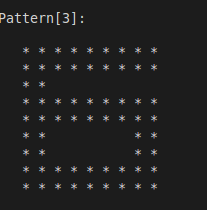
\includegraphics[width=.4\linewidth]{sixd.png}
  \caption{Training pattern for 6}
  \label{fig:sixt}
\end{subfigure}%
\begin{subfigure}{.5\textwidth}
  \centering
  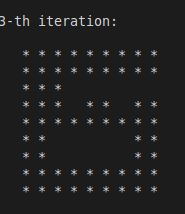
\includegraphics[width=.4\linewidth]{six3.png}
  \caption{After error rate increased}
  \label{fig:six3}
\end{subfigure}
\caption{Output for pattern 6}
\label{fig:one}
\end{figure}

\begin{figure}
\centering
\begin{subfigure}{.5\textwidth}
  \centering
  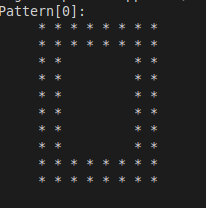
\includegraphics[width=.4\linewidth]{zerot.png}
  \caption{The pattern 0 for training}
  \label{fig:zerot}
\end{subfigure}%
\begin{subfigure}{.5\textwidth}
  \centering
  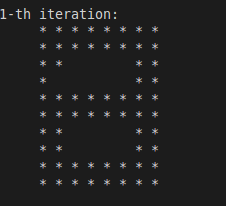
\includegraphics[width=.4\linewidth]{zero3.png}
  \caption{After error rate increased}
  \label{fig:zero3}
\end{subfigure}
\caption{Output for pattern 0}
\label{fig:two}
\end{figure}


From the Figure-1 and Figure-2 we although reconstructed the digit 6 succesfully, the
pattern 0 has been overlapped with some other digit. 

\subsection{Discussion and Conlusion}
It is to be noted that, when we store more patterns we get interception between 
them (it’s called a crosstalk) and each pattern add some noise to other patterns.

From the given resource and slide we know that the capacity of a network is
0.15N where N is the number of neuron. Saving more than \textbf{0.15N} pattern in the 
neuron will result in confusing the network and saturated. But here the reason
of the such near mis-match was  the \textbf{spurious minima} of the hopfield
network. Few points have been presented below to depict the side effects of the
network due to increase noise rate.
\begin{itemize}
  \item \textbf{The spurious minima} of the network occurs \textbf{when two 
      nearby energy minima combine to make a new minima in wrong place}. 
  \item Increasing the noise rate to a certain extend causes the network
    to converge to a \textbf{new minima}. As a result the network fails to
    retrieve it's saved pattern. The network gets stucked to the saddle 
    point which is depicted in the Figure 3.
  \item If the rate of noise is limited to a certain extent the network usually
    succesfully finds the attractor after few iteration. In this case 0.05 to
    0.30 was the limit. Beyond that it gets stucked to new minima. 
\end{itemize}


\begin{figure}
\centering
\begin{subfigure}{.5\textwidth}
  \centering
  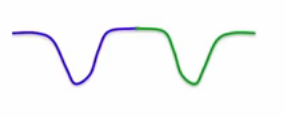
\includegraphics[width=.4\linewidth]{sp.png}
  \caption{Two energy minima for two different patterns}
  \label{fig:sp}
\end{subfigure}%
\begin{subfigure}{.5\textwidth}
  \centering
  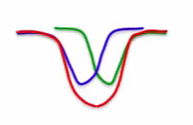
\includegraphics[width=.4\linewidth]{sp2.png}
  \caption{Two energy minima overlapped due to error and merged to create
  single engery minima}
  \label{fig:six3}
\end{subfigure}
\caption{A simple example of spurious minima problem}
\label{fig:three}
\end{figure}

In the figure 3 the blue curve is the energy minima for one pattern and the
green for another. But after error rate has been increased it is possible that
during the recall the energy minima of the corrupted image overlaps with the
engery minima of completely different pattern. Thus failing to recreate the
original intended pattern. So the new energy minima is the \textbf{red} curve
which is a mixture of two patterns. This kind of problem also occurs when the
network is taught a lot of patterns more than its limit \i.e. more than 0.15N. 


**\textbf{The image of figure -3 for spurious minima has been taken from the video lecture of Sir
Geoffrey Hinton}


\end{document}
